\section{Auswertung}
\label{sec:Auswertung}
\paragraph{Justage} 
Nach der Justage der Appartur wurden folgenden Shimparamter eingestellt.
\begin{equation*}
x = -1,58 \quad y = -6,6 \quad z = 3,68 \quad Z^2 = -1,72	
\end{equation*}
Die Frequenz wurde auf \SI{21,71524}{\mega\Hz} eingestellt. Die Phase auf 
\SI{161}{\degree} einjustiert. Die Periode zwischen den Pulsen wurde 
\SI{11}{\second} gewählt. Für die Messung von $T_2$ und der Diffusionskonstante 
jedoch auf \SI{8}{\second} nachjustiert.

\subsection{Bestimmung der Relaxationszeit \texorpdfstring{$T_1$}{math}}
Zur Messung der Relaxationszeit $T_2$ wurder die induzierte Spannung gegen den varrierten 
Pulsabstand $\tau$ gemessen und in Abbildung \ref{fig:T1} aufgetragen. Nach \cite{Anleitung} 
ist der Zusammenhang der beiden Messgrößen gegeben über 
\begin{equation}
U_z = U_0 \cdot \left( 1-2\exp \left( -\frac{\tau}{T_1} \right) \right) + b	\; ,
\end{equation}
dabei bezeichnet $U_z$ die induzierte Spannung. Durch nicht-lineare Ausgleichsrechnung 
ergibt sich $U_0 = \SI{0.667(4)}{\volt}$, $b = \SI{-0.007(4)}{\volt}$ und $T_1 = \SI{2.28(3)}{\second}$. 
\begin{figure}
  \centering
  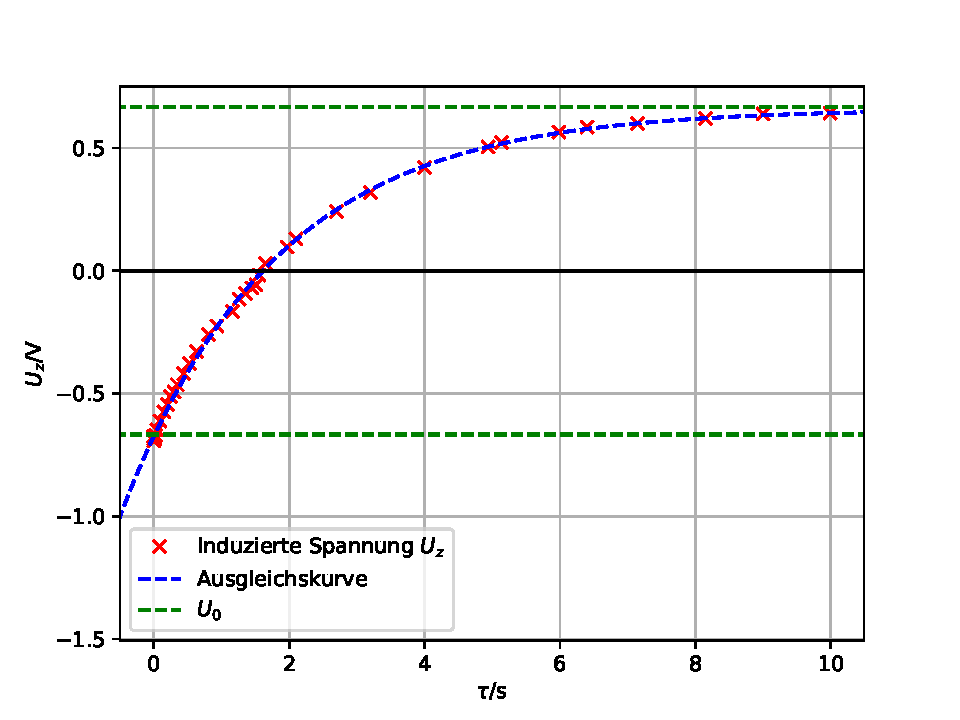
\includegraphics[height = 10cm]{plots/T1plot.pdf}
  \caption{Induzierte Spannung gegen den Pulsabstand aufgetragen.}
  \label{fig:T1}
\end{figure}

\subsection{Bestimmung der Relaxationszeit \texorpdfstring{$T_2$}{math}}
\paragraph{Meiboom-Gill-Methode} Zur Bestimmung der Relaxationszeit $T_2$ wurde mit der Meiboom-Gill-Methode die 
Abbildung des Signals \ref{fig:MGMO} mit einem Oszillioskop erzeugt. Die dazugehörigen Werte wurden ausgelsen und die 
Spitzen des Signals wurden ermittelt. Aus den Werten wurden die Werte ermittelt, die die Einhüllende beschreiben, diese 
wurden logarithmetisiert und in der Abbildung \ref{fig:T2} dargestellt. Zudem wurde mit linearer Ausgleichsrechnung eine 
Ausgleichsgerade berechnet. Der Zusammenhang der Messgrößen ist über die Gleichung 

\begin{figure}
  \centering
  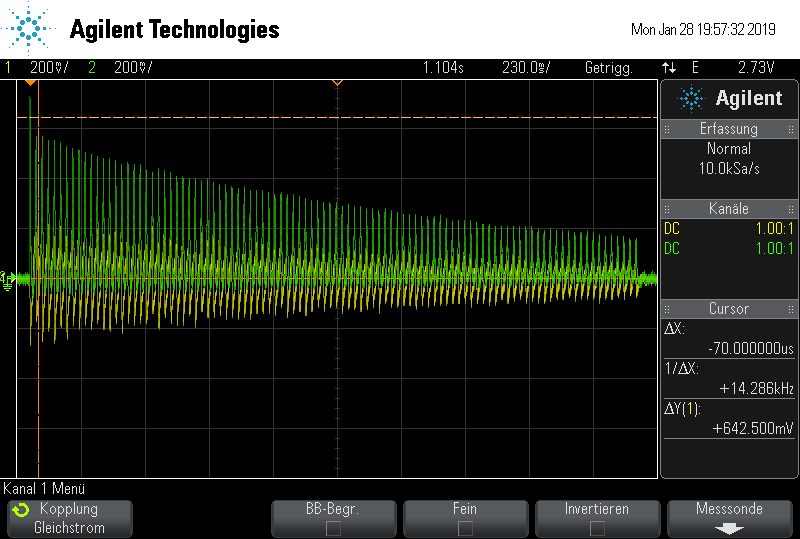
\includegraphics[height = 7cm]{plots/scope_1.png}
  \caption{Abbildung des Meiboom-Gill-Signals auf dem Oszilloskop.}
  \label{fig:MGMO}
\end{figure}
\begin{figure}
  \centering
  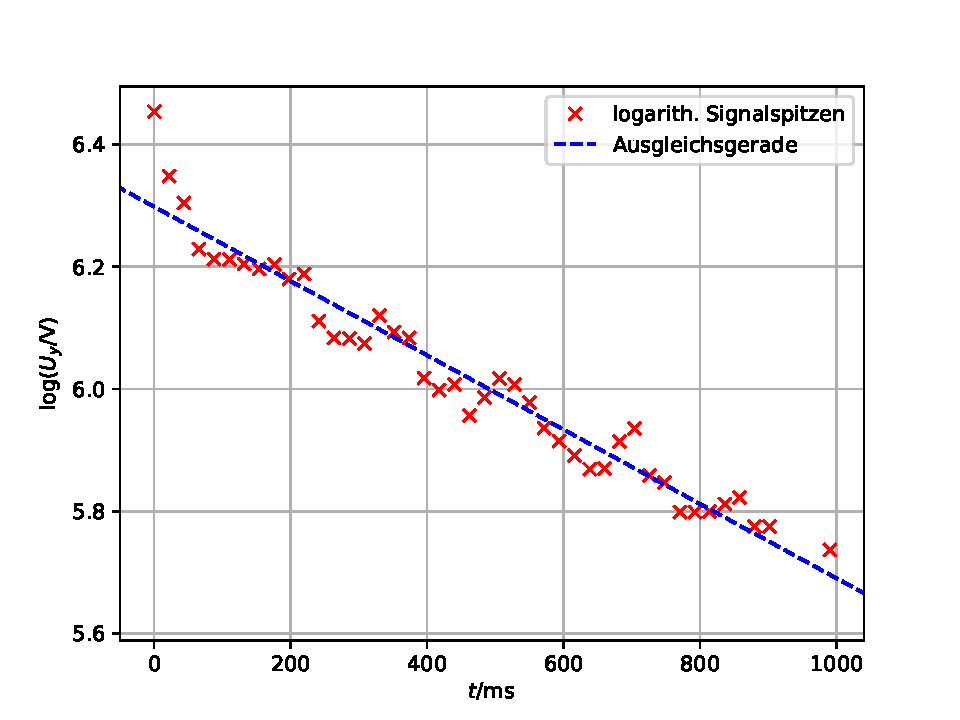
\includegraphics[height = 10cm]{plots/T2plot.pdf}
  \caption{Logarithmitisierte Einhüllende gegen den Pulsabstand.}
  \label{fig:plot}
\end{figure}


\paragraph{Carr-Purcell-Methode}
\subsection{Bestimmung der Diffusionskonstante}
\subsection{Bestimmung der Viskosität}
\subsection{Bestimmung der Molekülradien}
